\chapter{Noise Generation}
\label{NoiseGen}
Noise generation is one of the most essential topic in procedural content generation. Noise is often used in computer graphics and special effects, but is also used to randomly create or modify procedurally generated worlds. Noise generation can be a very complicated topic to fully understand. We will in this chapter look into some of the most commonly known noises as well as how to use them and manipulate them.


\section{Perlin Noise}

Perlin noise is one of the most common used noises in computer graphics and special effects. Perlin noise was originally created by Ken Perlin\cite{KenPerlin} in 1985 while working on the movie Tron\cite{perlinnoise}. Perlin noise is also the noise that often is used or adapted upon to create other sorts of noises, or manipulating with noises.

As we have mentioned earlier we will use libnoise for this project and will there by not implement our own perlin noise, however this section should provide the idea about how to implement your own perlin noise, as well as how perlin noise in general works.

Perlin noise is created by adding multiple layers of noise together with different amplitude, the amount between the highest and the lowest peak value, and frequency, how often the value is changed\cite{perlinnoise2}. Values are randomly generated within the amplitude and frequency range as the example in \figref{fig:1DNoise} show. The final result from adding all the layers together will give a smooth noise pattern which then can be used to define low and high values\cite{NoiseMachineMakingNoise}. To demonstrate the process we have 6 layers of noise in \figref{fig:1DNoise}, and when taking the sum of all graphs we end up with a graph shown in \figref{fig:1DNoiseResult}

\begin{figure}[H]
	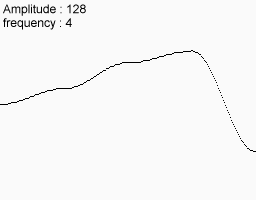
\includegraphics[width=0.32\linewidth]{img/noise_a}
	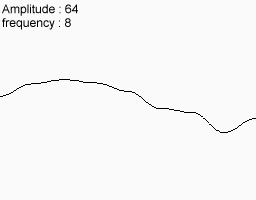
\includegraphics[width=0.32\linewidth]{img/noise_b}
	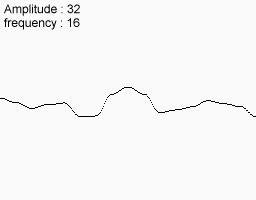
\includegraphics[width=0.32\linewidth]{img/noise_c}
	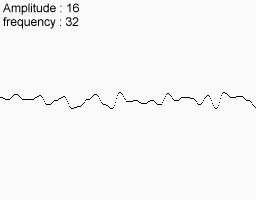
\includegraphics[width=0.32\linewidth]{img/noise_d}
	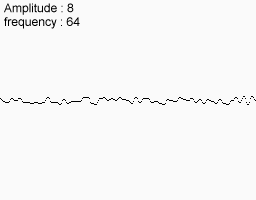
\includegraphics[width=0.32\linewidth]{img/noise_e}
	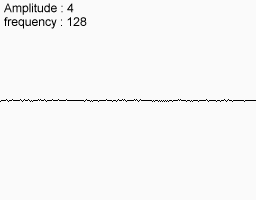
\includegraphics[width=0.32\linewidth]{img/noise_f}
	\centering
	\caption{6 graphs showing different layers of noise with the amplitude getting halved and frequency doubled for every new layer to finally create the result seen in \figref{fig:1DNoiseResult} Images used is taken from \cite{perlinnoise2}.}
	\label{fig:1DNoise}
\end{figure}
\begin{figure}[H]
	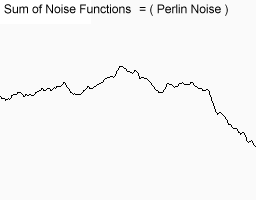
\includegraphics[width=0.5\linewidth]{img/perlin1}
	\centering
	\caption{The final graph result from the sum of all of the graphs shown in \figref{fig:1DNoise}. The image used is taken from \cite{perlinnoise2}.}
	\label{fig:1DNoiseResult}
\end{figure}

The exact same idea can be adapted to create 2 dimensional noise. In \figref{fig:2DNoise} we see the exact same that happened in \figref{fig:1DNoise} but in a 2 dimensional space rather than in 1 dimension. We have 6 different noise maps with different amplitude and frequency which is combined into a single noisemap which should give a smooth gradient transition between high and low values. All the black areas is typically representing the lowest values and white represent the highest values, however, in \figref{fig:2DNoise} case purple represents the high values.

\begin{figure}[H]
	
\includegraphics[width=0.135\linewidth]{img/perlin_a}
	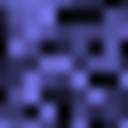
\includegraphics[width=0.135\linewidth]{img/perlin_b}
	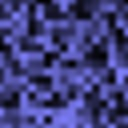
\includegraphics[width=0.135\linewidth]{img/perlin_c}
	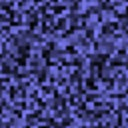
\includegraphics[width=0.135\linewidth]{img/perlin_d}
	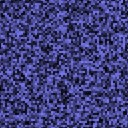
\includegraphics[width=0.135\linewidth]{img/perlin_e}
	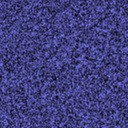
\includegraphics[width=0.135\linewidth]{img/perlin_f}
	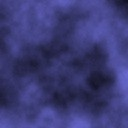
\includegraphics[width=0.135\linewidth]{img/p_128}
	\centering
	\caption{The images show layers of 2 dimensional noise with the frequency getting larger with the leftmost image being the lowest frequency. The Rightmost image is the final noise generated from the 6 other images. Images used is taken from \cite{perlinnoise2}.}
	\label{fig:2DNoise}
\end{figure}

Perlin noise offers multiple parameters that we can change, to modify the output noise. The first and most important is octaves which defines how many layers of noise should be created to produce the final result. In \figref{fig:1DNoise} and \figref{fig:2DNoise} the octaves is 6, as there is 6 noise maps that is used to generate the final result. We also need a parameter to define our starting frequency, and the frequency multiplier, which is often referred to as persistence. In \figref{fig:1DNoise} we have a persistence of 2 as the frequency is double on each octave and the amplitude halved. In libnoise persistence does however only control the amplitude, and libnoise introduces yet another parameter called lacunarity which in libnoise is used as the frequency multiplier\cite{libnoisePerlin}.

The last thing needed to make perlin noise is an interpolation function. Interpolation is a way of connecting the randomly generated points to each other. The first is linear interpolation, which is demonstrated in \figref{fig:1a}, the connections is direct and the result may not be very realistic. To improve the result even more we could use a cosine interpolation as seen in \figref{fig:1b}. We now have somewhat realistic curves, but we can improve the curve even more by making a cubic interpolation as shown in \figref{fig:1c}. Cubic interpolation is often used as it provides the most realistic curves between multiple points. The last step is an optional step that can make the output noise slightly more realistic by smoothing the curve so that the peak values get reduced as can be seen in \figref{fig:1d}.


\begin{figure}[H]
	\begin{minipage}[b]{.5\linewidth}
		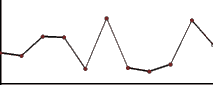
\includegraphics[width=0.95\linewidth]{img/m_inter1}
		\subcaption{Linear interpolation}
		\label{fig:1a}
		%\begin{equation*}
		%	a*(1-x) + b*x
		%	\label{linear}
		%\end{equation*} 
	\end{minipage}
	\begin{minipage}[b]{.5\linewidth}
		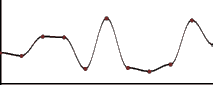
\includegraphics[width=0.95\linewidth]{img/m_inter2}
		\subcaption{Cosine interpolation}
		\label{fig:1b}
		%\begin{equation*}
		%	(1 - cos(x * \pi)) * .5
		%	\label{Cosine}
		%\end{equation*} 
	\end{minipage}
	\begin{minipage}[b]{.5\linewidth}
		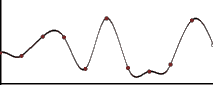
\includegraphics[width=0.95\linewidth]{img/m_inter4}
		\subcaption{Cubic interpolation}
		\label{fig:1c}
	\end{minipage}%
	\begin{minipage}[b]{.5\linewidth}
		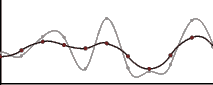
\includegraphics[width=0.95\linewidth]{img/m_inter6}
		\subcaption{Smoothed noise}
		\label{fig:1d}
		%\begin{equation*}
		%	a*(1-x) + b*x
		%	\label{linear}
		%\end{equation*} 
	\end{minipage}%

	\centering
	\caption{The images show 3 types of interpolation. \figref{fig:1a} shows Linear interpolation, \figref{fig:1b} shows Cosine interpolation, \figref{fig:1c} shows Cubic interpolation. \figref{fig:1d} is a last optional step that smoothen the final result such that the peaks get reduced. All images used is taken from \cite{perlinnoise2}.}
	\label{fig:interpolation}
\end{figure}

Example usage of perlin noise, other than for what we already have mentioned, could be real time generation of ocean waves, weather effect including clouds, rain, or storms.


\section{Voronoi Diagram}
\label{VoronoiDiagram}
Voronoi noise, or more commonly known as voronoi diagram, is a diagram built up by multiple voronoi cells. A Voronoi cell is a region containing all the points that are closer to a specific seed point than to any other seed point\cite{libnoiseVoronoi}. In \figref{fig:Voronoi} we see examples of two voronoi diagrams \figref{fig:2a} being a diagram with low displacement, meaning there will be fewer points, and \figref{fig:2b} has higher displacement and thereby creating more seed points.

There is multiple algorithms for generating voronoi diagrams, however one of the fastest is fortune's algorithm, made by Steven Fortune for his paper "A sweepline algorithm for Voronoi diagrams"\cite{VoronoiSweepLine}. In our case we use the libnoise libary for noise generation and libnoise does not state which algorithm they are using for voronoi diagrams.

\begin{figure}[H]
	\begin{minipage}[b]{.48\linewidth}
		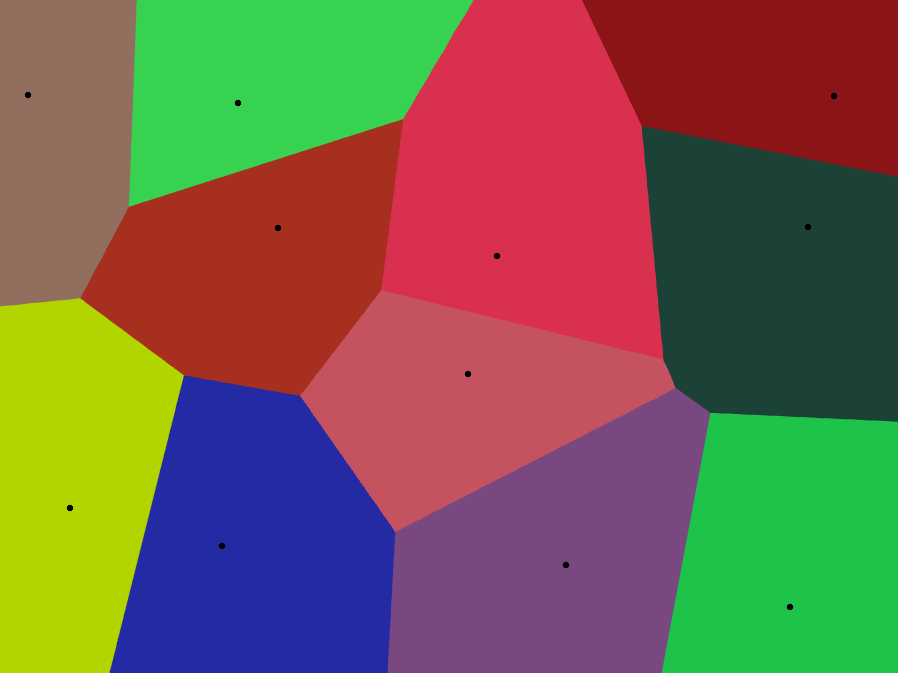
\includegraphics[width=0.95\linewidth]{img/VoronoiDiagramSmall}
		\subcaption{Low displacement voronoi diagram.}
		\label{fig:2a}
	\end{minipage}
	\begin{minipage}[b]{.48\linewidth}
		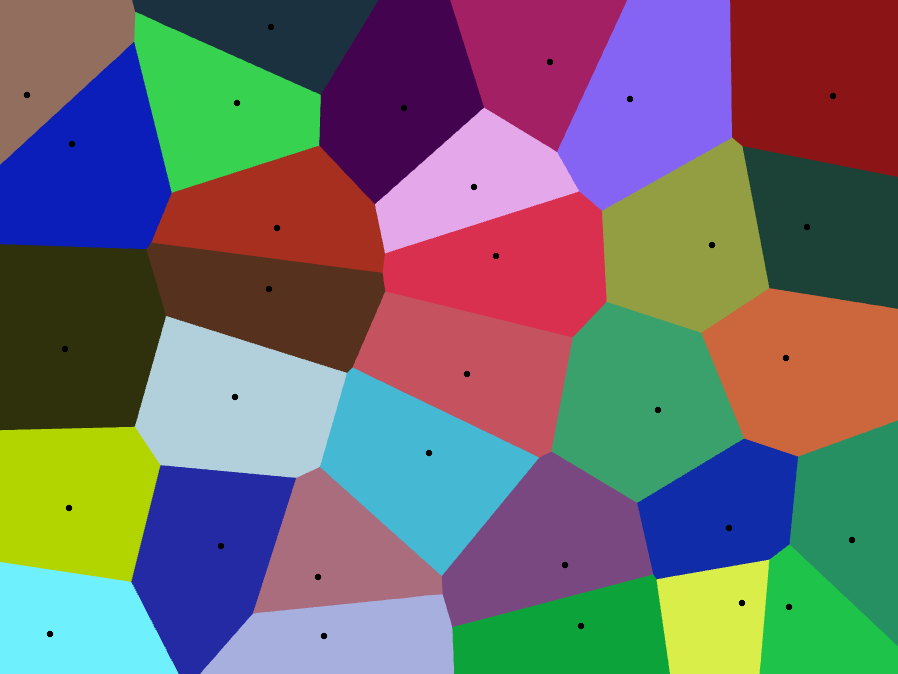
\includegraphics[width=0.95\linewidth]{img/VoronoiDiagramBig}
		\subcaption{High displacement voronoi diagram.}
		\label{fig:2b}
	\end{minipage}
		\centering
		\caption{The images shows 2 different displacements of a voronoi diagram.}
		\label{fig:Voronoi}
\end{figure}

There is multiple ways voronoi diagrams can be used in games, and one way of using it in procedural content generation could be to use voronoi diagrams to divide areas into regions, states, biomes, or territories. If we look at \figref{fig:Voronoi} each voronoi cell, or individual color, serves as an individual region. Another usage seen in 3D and games are shattering effects. In \figref{fig:VoronoiShatering} we seen an example of a voronoi shattering on a 3D object using the larmor-physx\cite{larmor-physx} plugin.

\begin{figure}[H]
	\begin{minipage}[b]{.49\linewidth}
		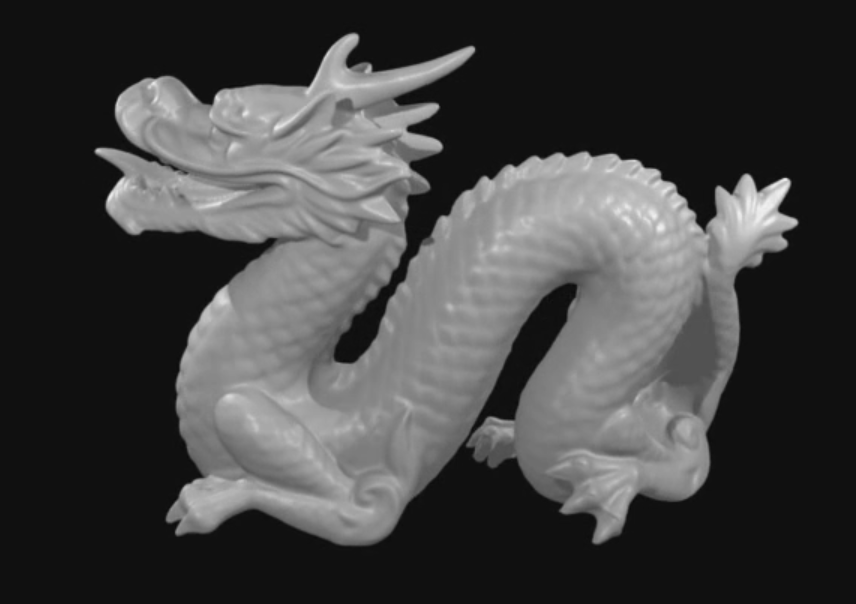
\includegraphics[width=0.95\linewidth]{img/VoronoiShatter1}
		\subcaption{A 3D model of a dragon figuette before any voronoi alterations.}
		\label{fig:3a}
	\end{minipage}
	\begin{minipage}[b]{.49\linewidth}
		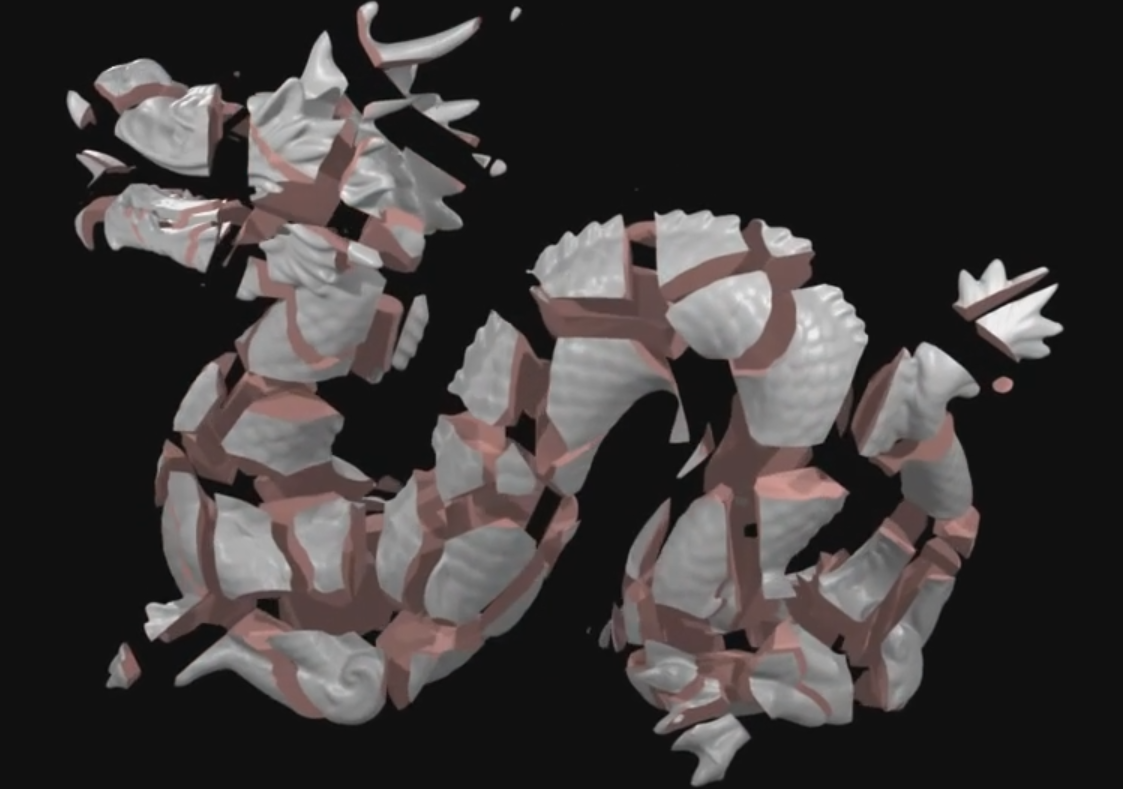
\includegraphics[width=0.95\linewidth]{img/VoronoiShatter2}
		\subcaption{The same dragon as in \figref{fig:3a} with voronoi shattering.}
		\label{fig:3b}
	\end{minipage}
	\centering
	\caption{The image shows a 3D figure being shattered using voronoi diagrams to determine the shatter points.}
	\label{fig:VoronoiShatering}
\end{figure}

Voronoi diagrams have many other usages which includes everything from Archeology to Zoology which is described in details at\cite{VoronoiDiagrams:Applications}. We will not go into much details about unrelated usages of voronoi diagrams, however some of them could possibly be adapted upon in games. 

It should also be mentioned that voronoi diagrams should not be confused with it's almost identical noise called Worley noise. Worley noise was made by Steven Worley for his paper "A Cellular Texture Basis Function" \cite{worley} and it is generated in a similar way to voronoi, but rather than creating a region from all points closest to a seed point, it creates a gradient color shift where the closer to a seed point the higher or lower the value as demonstrated in \figref{fig:worleynoise}. libnoise does have a similar, but not exact, way of generating voronoi maps by having the seed point be the lowest value in a region.

\begin{figure}[H]
	\centering
	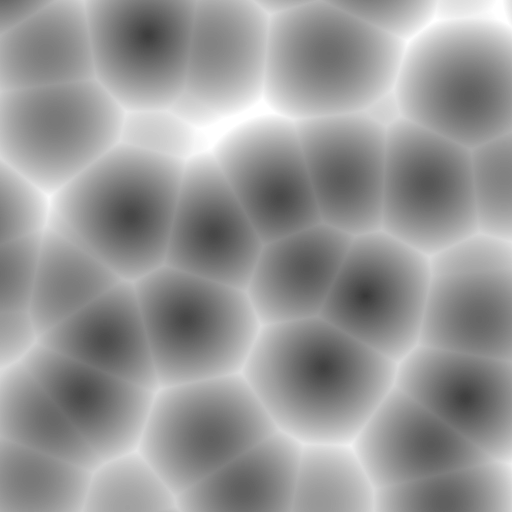
\includegraphics[width=0.5\linewidth]{img/worley_noise}
	\caption{The images shows an example of Worley noise.}
	\label{fig:worleynoise}
\end{figure}


\section{Billow Noise and Ridged Noise}
\label{brnoise}
Billow noise and Ridged noise, or RidgedMultiFractual Noise, are two other noises that are interesting for procedural content generation. Both noises look very similar to each other as can be seen in \figref{fig:BillowRidged}. Both noises are heavily based on perlin noise, and billow is almost identical to perlin noise with the only exception the each octave is modified by an absolute value\cite{libnoiseBillow}\cite{NoiseMachineMakingNoise}. Billow noise is a great noise to use for creating for instance cloud systems.

Ridged noise is also based on perlin noise and is also generated almost the same way as perlin noise, however like billow noise, ridged noise's octaves are modified by an absolute value\cite{NoiseMachineMakingNoise}, but also however the persistence parameter is left out as it is based on the previously generated octaves\cite{libnoiseRidged}. Ridged noise has different usages, one of them is using it to generate craggy mountains or rivers. Another interesting usage is to generate cave like structures which especially is used in voxel engines with procedural content generation, eg. Minecraft.

\begin{figure}[H]
	\begin{minipage}[b]{.49\linewidth}
		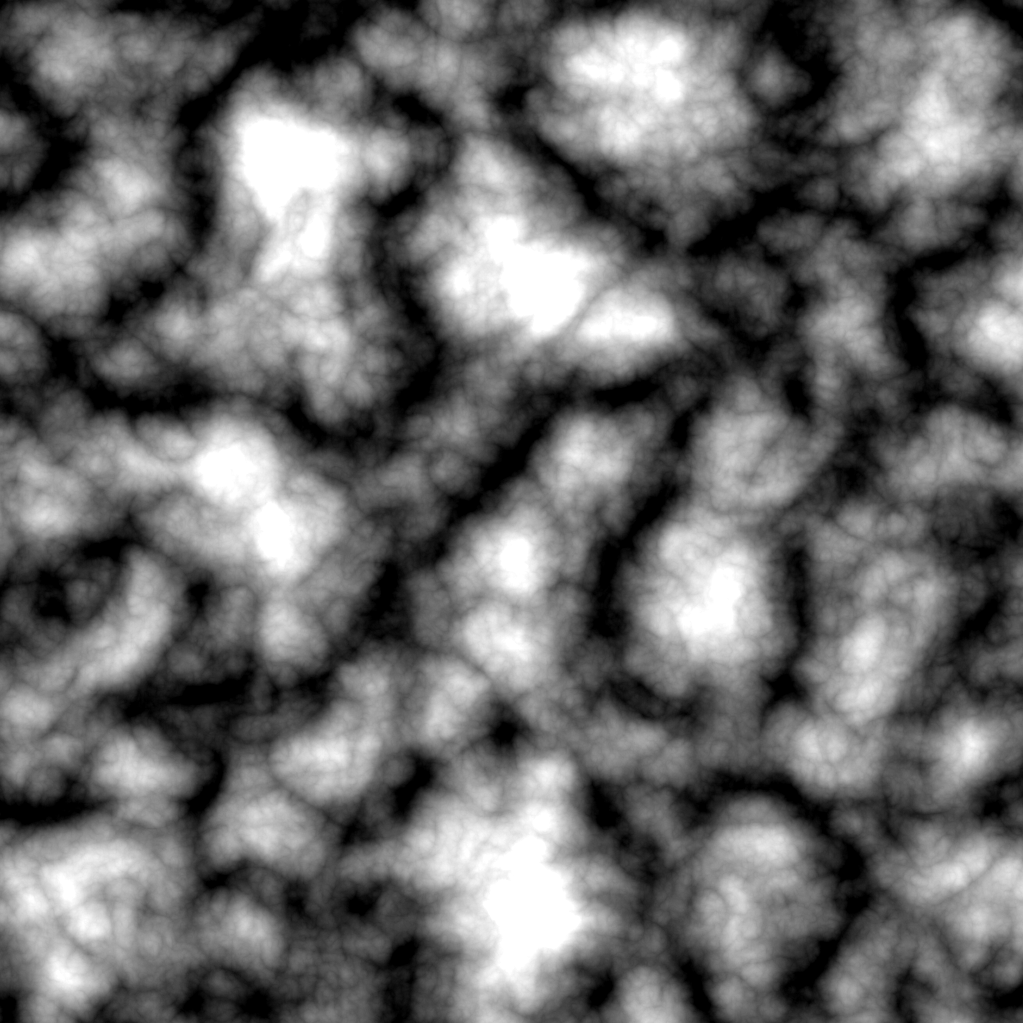
\includegraphics[width=0.95\linewidth]{img/Billow}
		\subcaption{Billow Noise}
		\label{fig:4a}
	\end{minipage}
	\begin{minipage}[b]{.49\linewidth}
		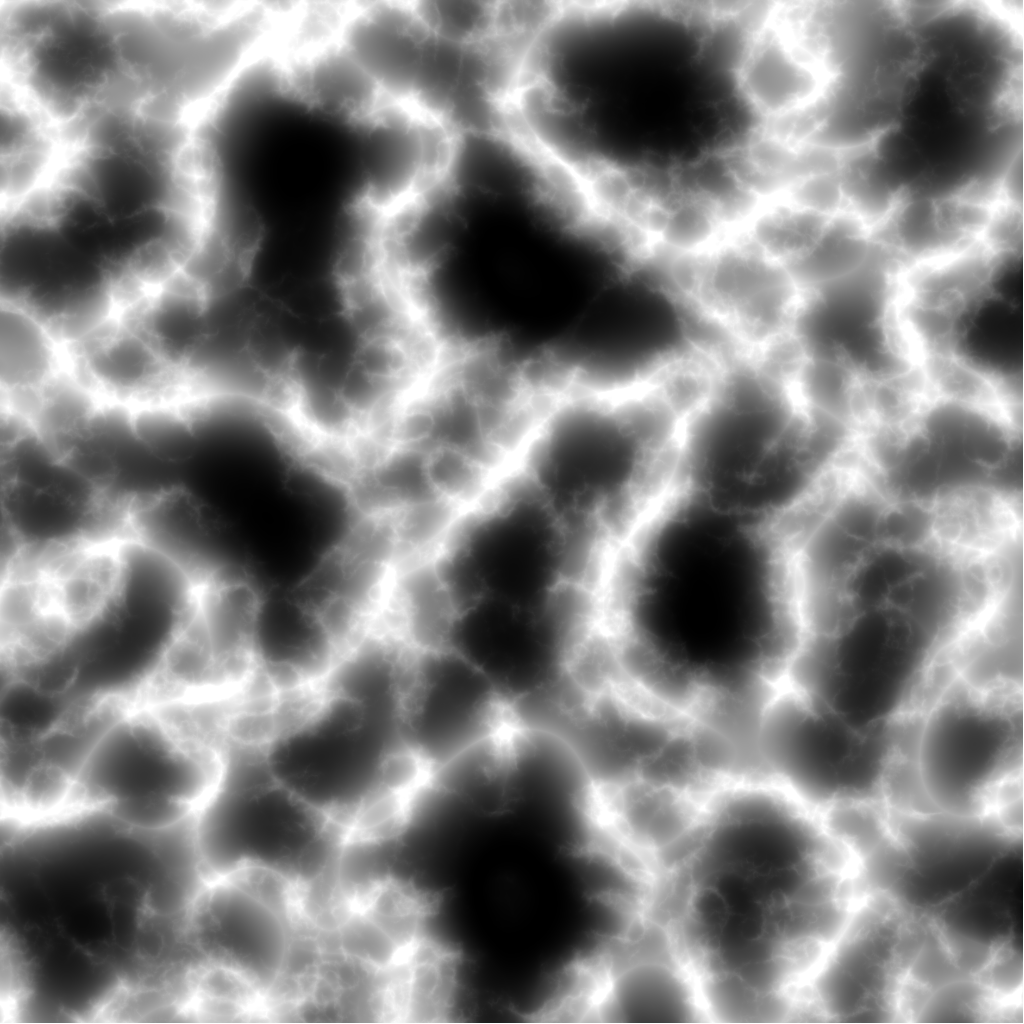
\includegraphics[width=0.95\linewidth]{img/Ridged}
		\subcaption{Ridged Noise}
		\label{fig:4b}
	\end{minipage}
	\centering
	\caption{The figure show an example of billow and ridged noise both generated with the exact same parameters, which results in both noise maps almost looks inversed of each other.}
	\label{fig:BillowRidged}
\end{figure}


\section{Noise Manipulating}
\label{NoiseManipulating}
Besides generating noise, different operations to modify and combine noises together, is something that is very useful. libnoise already contains multiple operator modules that can add, substitute, multiply, and many others, noises together to create a mathematical combination of 2 noises. Here we will look into a few examples of how these operators can be used to modify the noise maps.

A prime example used in real life like procedural generated worlds, is using a heightmap, generated from perlin noise, and a latitude map created from either to decide temperature by adding those two together as we demonstrate in \figref{fig:Temperature} and will be describing more in depth in section \ref{WorldGenerator}.

\begin{figure}[H]
	\begin{minipage}[b]{.32\linewidth}
		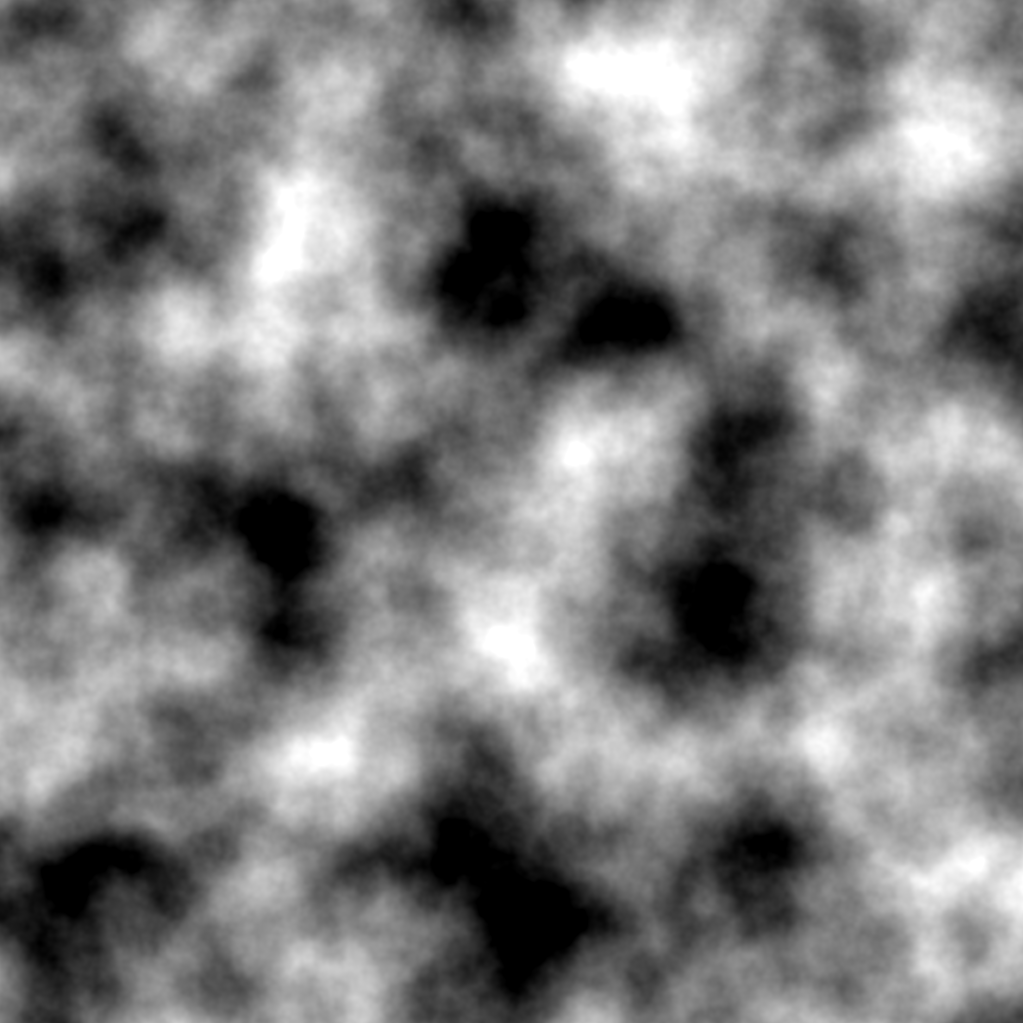
\includegraphics[width=0.95\linewidth]{img/Perlin}
		\subcaption{Heightmap generated from perlin noise.\\\\}
		\label{fig:5a}
	\end{minipage}
	\begin{minipage}[b]{.32\linewidth}
		
\includegraphics[width=0.95\linewidth]{img/Latitude}
		\subcaption{Latitude map generated with cosine or linear gradient.\\}
		\label{fig:5b}
	\end{minipage}
	\begin{minipage}[b]{.32\linewidth}
		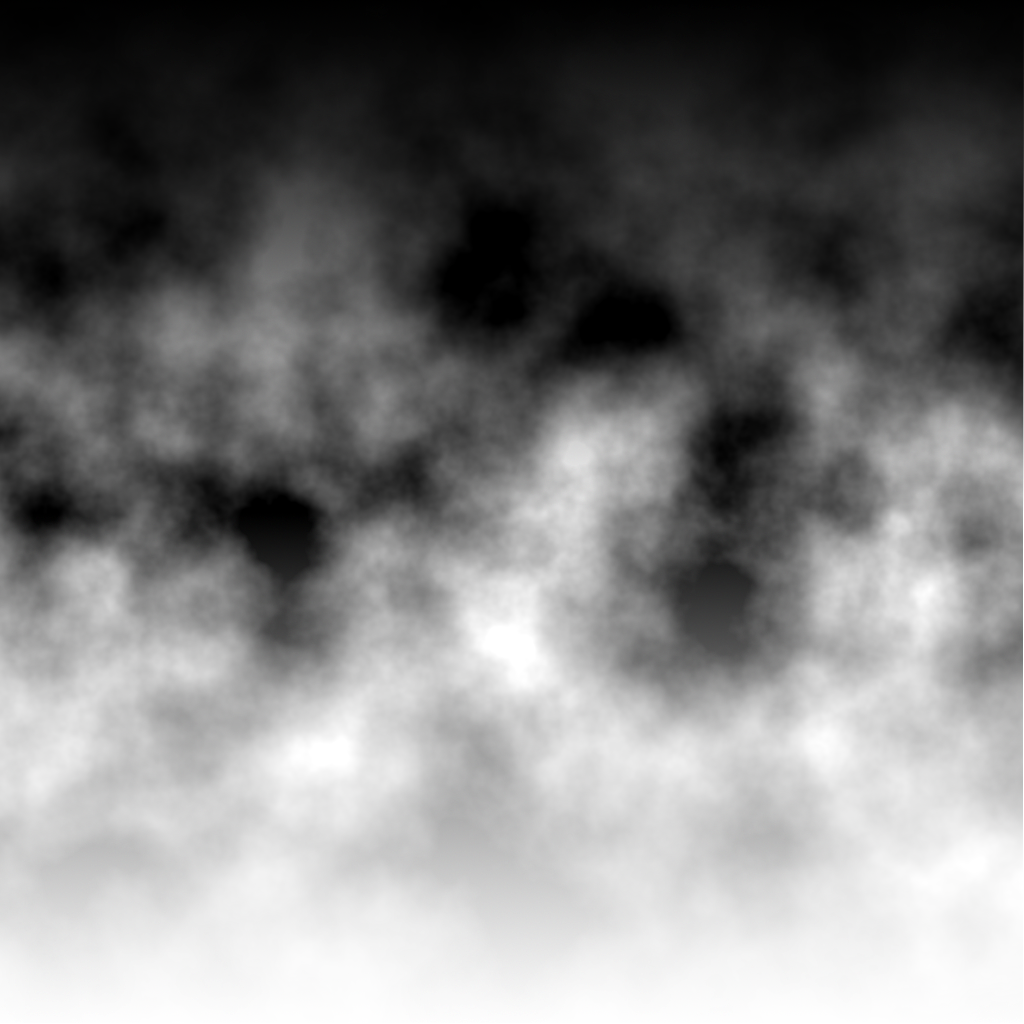
\includegraphics[width=0.95\linewidth]{img/Temperature}
		\subcaption{The resulting Temperature map by adding \figref{fig:5a} and \figref{fig:5b} together.}
		\label{fig:5c}
	\end{minipage}
	\centering
	\caption{The figure shows an example of adding two noises together in libnoise. The two noises combined results in a temperature map, and high points as well as polar areas has lower temperatures.}
	\label{fig:Temperature}
\end{figure}

As we mentioned in section \ref{brnoise} ridged noise can be used to generate cave systems. This can be done by decreasing all low values within a range but leave the high numbers unchanged. A way of doing this is to simply take an entirely black mask and add it once or multiple times to achieve what is seen in \figref{fig:Caves}

\begin{figure}[H]
	\begin{minipage}[b]{.32\linewidth}
		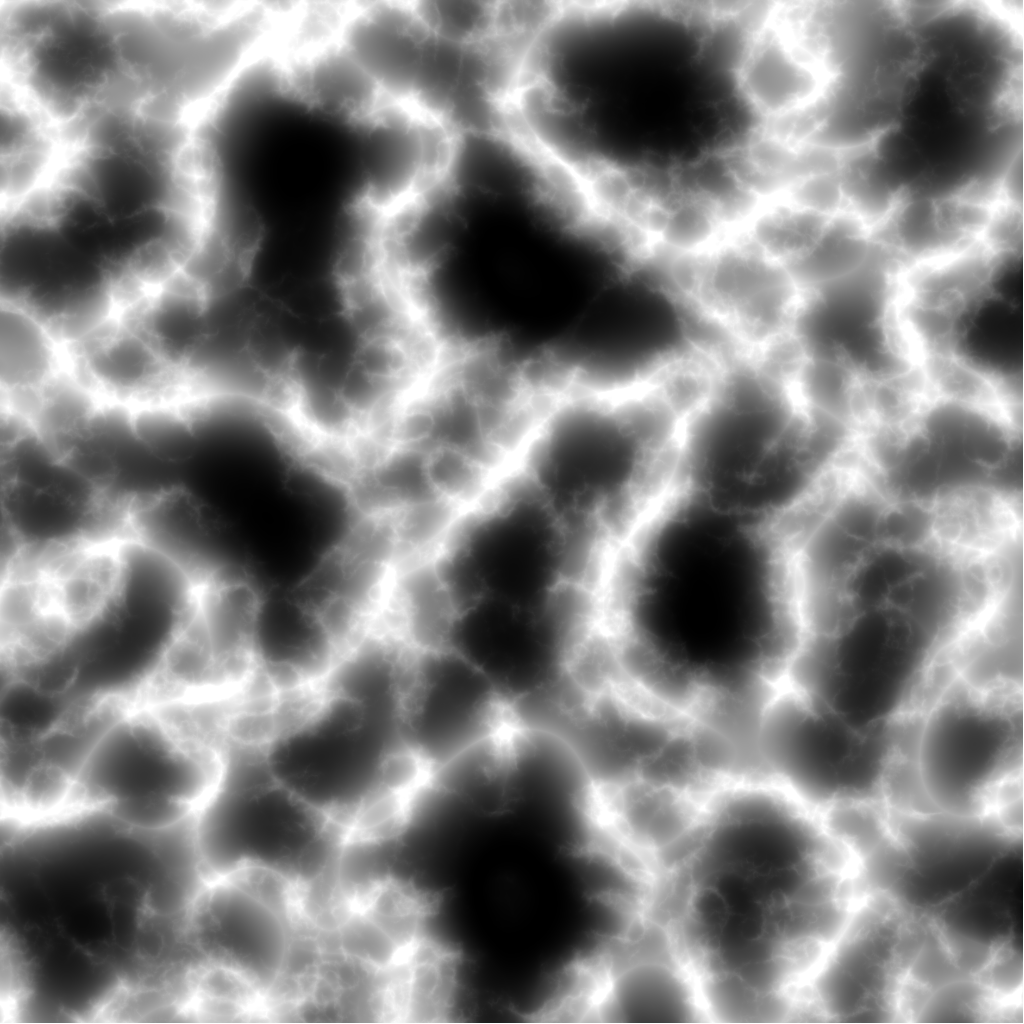
\includegraphics[width=0.95\linewidth]{img/Ridged}
		\subcaption{Ridged map generated from Ridged noise. \\\\}
		\label{fig:6a}
	\end{minipage}
	\begin{minipage}[b]{.32\linewidth}
		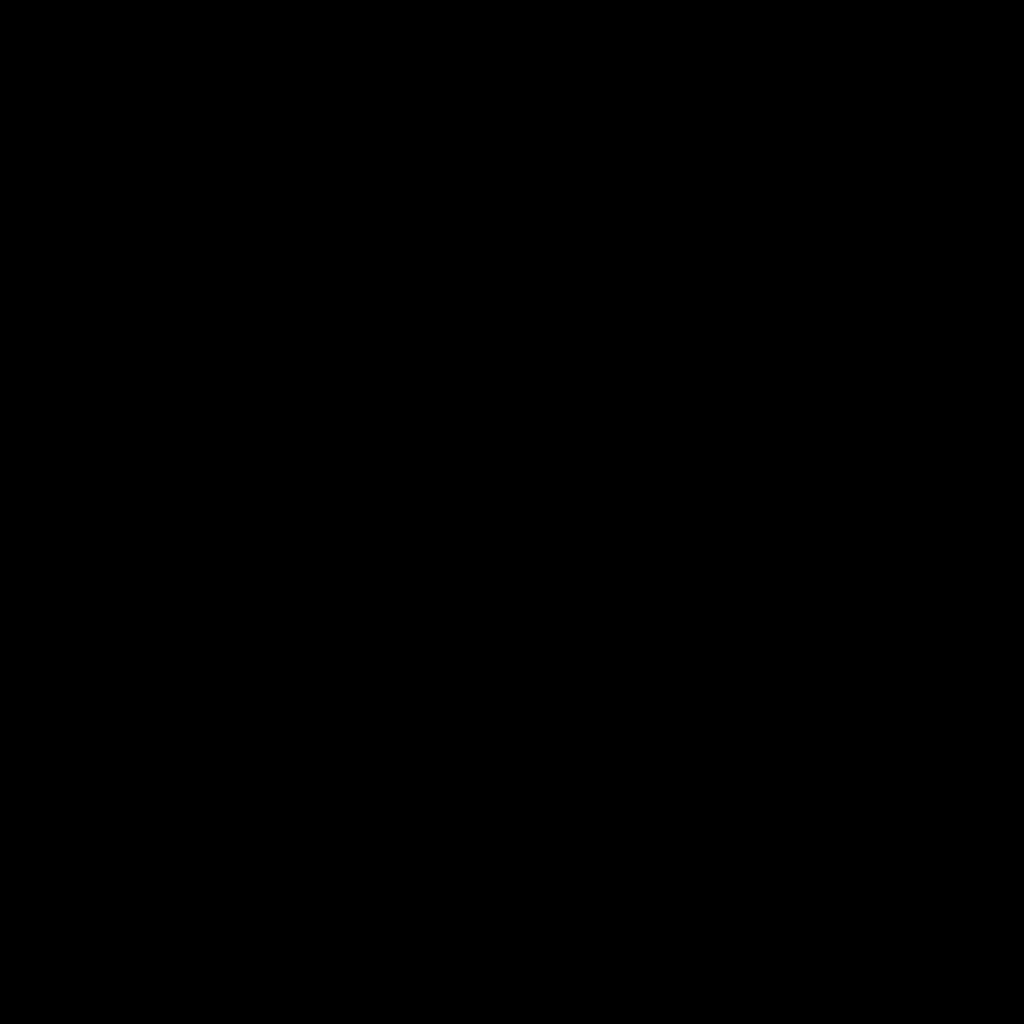
\includegraphics[width=0.95\linewidth]{img/BlackMask}
		\subcaption{A black mask texture used to decrease values lower values.\\}
		\label{fig:6b}
	\end{minipage}
	\begin{minipage}[b]{.32\linewidth}
		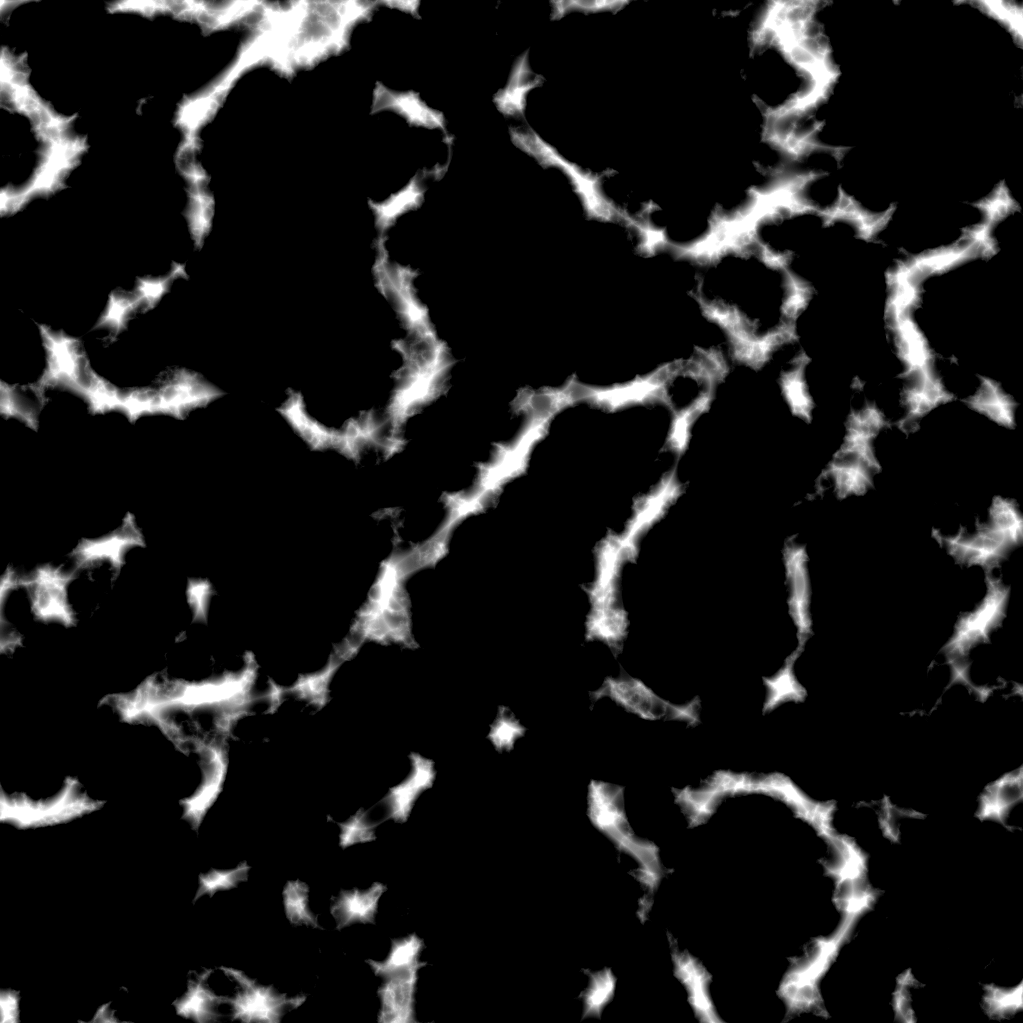
\includegraphics[width=0.95\linewidth]{img/Caves}
		\subcaption{The resulting cave map after \figref{fig:5b} have been masked twice onto \figref{fig:5a}.}
		\label{fig:6c}
	\end{minipage}
	\centering
	\caption{The figure shows an example on how cave systems in voxel engines can be made by masking a entirely black texture onto a ridged noise map.}
	\label{fig:Caves}
\end{figure}